\chapter{\label{app:ex}Software demonstration}

For the following two worked examples, we assume that the following imports 
have been made.

\begin{verbatim}
>>> import numpy as np
>>> from scipy import stats
>>> import matplotlib.pyplot as plt
\end{verbatim}

You will also need to have \texttt{permute} version \texttt{0.1a1} installed.

\begin{verbatim}
>>> import permute
>>> permute.__version__
'0.1a1'
\end{verbatim}

Note that this is an \emph{alpha} release, so we are making no claims
regarding the stability of our package structure or call signatures.  We do not
have plans to break our API, but we are allowing ourselves to continue refining
our API as we gain experience using the package and continue adding new
functionality.  However, the following example sessions will give you an idea
of what working with \texttt{permute} is like.

\section*{Two sample permutation test}

There is growing evidence of gender bias in student evaluations of teaching.
To address the question ``Do students give higher ratings to male teachers?,''
an online experiment was done with two professors, one male and one female
\cite{macnell2014s}.  Each professor taught two sections. In one section, they
used a male name.  In the other, they used a female name. The students didn't
know the teacher's real gender.  We test whether student evaluations of
teaching are biased by comparing the ratings when the professor used a male
name versus a female name.

First let us consider the parametric two-sample t-test.  In this case, our
test statistic is
\begin{align*}
t &= \frac{\text{mean(rating for M-identified prof) - mean(rating for F-identified prof)}}{\sqrt{\text{pooled SD of ratings}}}
\end{align*}
For the two-sample t-test, the null hypothesis is that the reported/perceived
teacher gender has no effect on teacher ratings.  The alternative hypothesis
is that teacher ratings differ by reported/perceived teacher gender.  For the
two-sample t-test to be valid, we require the following assumptions:
\begin{itemize}
\item Ratings are normally distributed.  (But they are on a Likert 1-5 scale,
      which is definitely not normal.)
\item Noise is zero-mean and constant variance across raters.  (How should we interpret
      ``noise'' in this context?  Besides constant variance is not plausible: some
      raters might give a range of scores, other raters might always give 5.)
\item Independence between observations. (Students might talk about ratings with
      their peers in the class, creating dependence.)
\end{itemize}

Despite the problematic assumptions we are required to make, let's temporarily
assume they hold and calculate a ``p-value'' anyway.

\begin{verbatim}
>>> from permute.data import macnell2014
>>> ratings = macnell2014()
>>> maleid = ratings.overall[ratings.taidgender==1]
>>> femaleid = ratings.overall[ratings.taidgender==0]
>>> df = len(maleid) + len(femaleid) - 2
>>> t, p = stats.ttest_ind(maleid, femaleid)
>>> print 'Test statistic:', np.round(t, 5)
Test statistic: 1.54059
>>> print 'P-value (two-sided):', np.round(p, 5)
P-value (two-sided): 0.1311
\end{verbatim}
Note that the computed ``p-value'' is above the standard cut-offs for
reporting significance in the literature.

For the permutation test we can use the same test statistic, but we will
compute the p-value by randomly sampling the exact distribution of the test
statistics.  The null hypothesis is that reported/perceived teacher gender has
no effect whatsoever on ratings---as if ``male'' and ``female'' are randomly
assigned labels.  The alternative hypothesis is that reported/perceived teacher
gender has some effect on ratings.  The only assumption we need to make is that
randomization is fair and independent across units.  This can be verified
directly from the experimental design.

\begin{verbatim}
>>> from permute.core import two_sample
>>> p, t, ci, dist = two_sample(maleid, femaleid, stat='t',
...                             interval='two-sided', keep_dist=True)
>>> print 'Test statistic:', np.round(t, 5)
Test statistic: 1.82159
>>> print 'P-value (two-sided):', np.round(p, 5)
P-value (two-sided): 0.04436
>>> print '95% Confidence Interval for the P-value', np.round(ci, 5)
95% Confidence Interval for the P-value [ 0.04309  0.04565]
\end{verbatim}

Not only is the use of this p-value justified (since our assumptions are
met), but its value is below the cut-off for significance commonly used.
Since the permutation test also returns the approximately exact distribution
of the test statistic, let's compare the actual distribution with the
$t$-distribution.

\begin{verbatim}
>>> n, bins, patches = plt.hist(dist, 20, histtype='bar')
>>> plt.axvline(x = t, color = 'red')
>>> x = np.linspace(stats.t.ppf(0.0001, df),
                    stats.t.ppf(0.9999, df), 100)
>>> plt.plot(x, stats.t.pdf(x, df)*(100000/2.0), lw=2, alpha=0.6, label='t pdf')
>>> plt.show()
\end{verbatim}

In Figure~\ref{fig:figure1}, you can see the simulated distribution of the test
statistic under the null with the $t$-distribution superimposed on it.

\begin{figure}
  \begin{centering}
    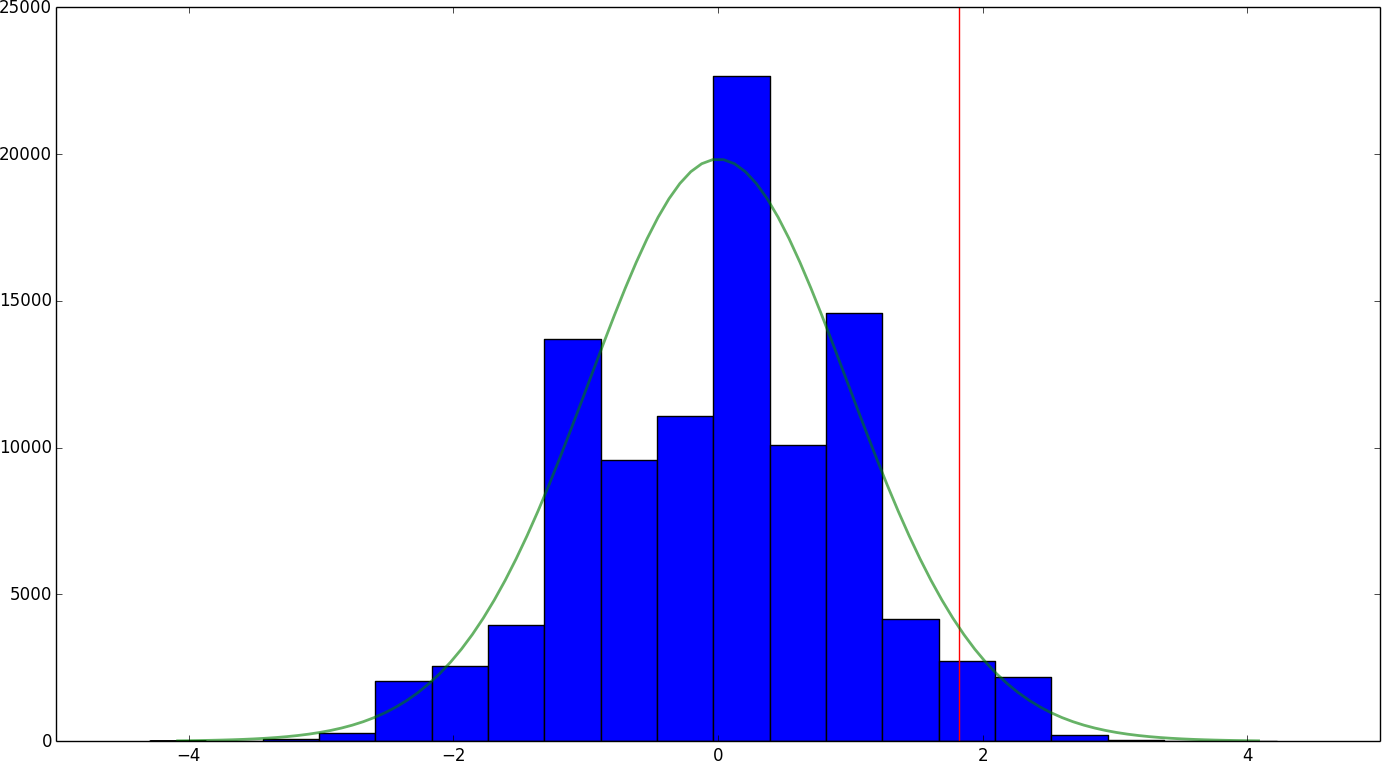
\includegraphics[width=.8\textwidth]{fig/figure_1.png}\par
  \end{centering}

  \caption{\label{fig:figure1}Permutation Null Distribution.}

\end{figure}

\section*{Stratified Spearman correlation permutation test}

To illustrate the use of one of our stratified tests, I will use fake
data similar to that used in \cite{boring2015}; we are unable to use
the actual data due to data privacy laws in France.

The scientific question of interest is now ``Do students' evaluations of
teachers measure teaching effectiveness?''  To answer this question, we were
able use final exam performance as a proxy for value added by
teacher---students have different teachers but take the same final exam.
Our null hypothesis is that there is no association between a student's final
exam performance and the rating they give their professor.  The alternative
hypothesis is that there is a positive association between a student's final
exam performance and the rating they give their professor.

There are 8 professors, each with multiple student ratings.  One might think
that a certain professor gets consistently high reviews because of something (e.g.,
gender, attractiveness, likeability) unrelated to teaching effectiveness.
Stratifying by professor allows us to assess teaching effectiveness for each
individual student.  The test statistic we use within groups is the Spearman
correlation.

\begin{verbatim}
>>> from permute.stratified import sim_corr
>>> evals = np.recfromcsv("SET2.csv")
>>> rho, plower, pupper, pboth, sim = sim_corr(x=evals.rating, y=evals.final,
...                                            group=evals.prof_id)
>>> print 'Test statistic:', np.round(rho, 5)
Test statistic: 0.94787
>>> print 'One-sided (upper) p-value:', np.round(pupper, 5)
One-sided (upper) p-value: 0.18
\end{verbatim}

Finally, I plot the simulated distribution of the test statistics under the null
conditioned on the observed data in Figure~\ref{fig:figure2}.

\begin{verbatim}
>>> n, bins, patches = plt.hist(sim, 40, histtype='bar')
>>> plt.axvline(x=rho, color='red')
>>> plt.show()
\end{verbatim}

\begin{figure}
  \begin{centering}
    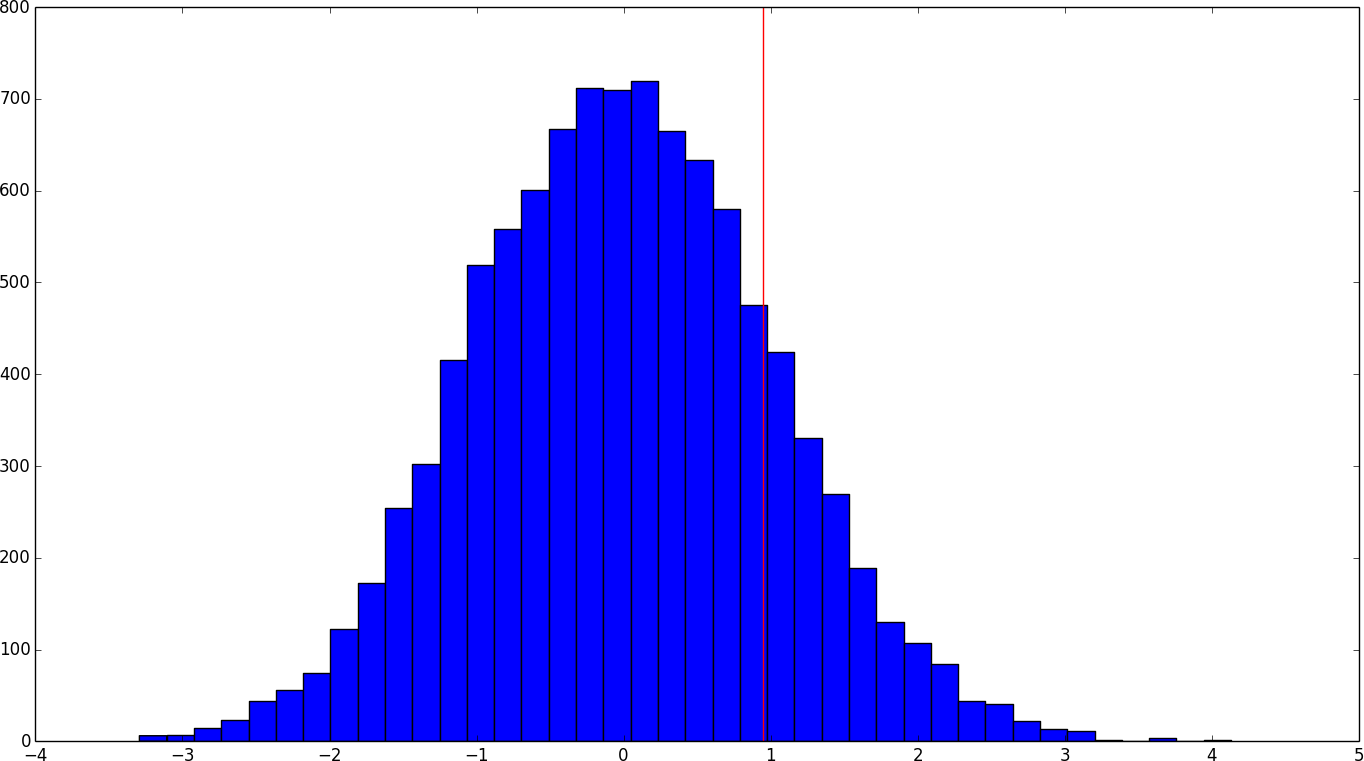
\includegraphics[width=.8\textwidth]{fig/figure_2.png}\par
  \end{centering}

  \caption{\label{fig:figure2}Permutation Null Distribution.}

\end{figure}

